\documentclass[a4paper,10pt,oneside,openany,uplatex]{jsbook}

%図表の個数などの設定.
\setcounter{topnumber}{4}
\setcounter{bottomnumber}{4}
\setcounter{totalnumber}{4}
\setcounter{dbltopnumber}{3}

\renewcommand{\topfraction}{.95}
\renewcommand{\bottomfraction}{.90}
\renewcommand{\textfraction}{.05}
\renewcommand{\floatpagefraction}{.95}

%使用するパッケージを記述.
\usepackage{amsmath, amssymb} %複雑な数式などを打つときに使用.
\usepackage{bm} %数式環境内で太字を使うときに便利.
%\usepackage{graphicx} %画像を挿入したり,テキストや図の拡大縮小・回転を行う.
\usepackage[dvipdfmx]{graphicx}
\usepackage{subfigure} %図を並べる(今はsubfigとかsubcaptionとかが推奨らしい.よく知らない)
\usepackage{verbatim} %入力どおりの出力を行う.
\usepackage{ascmac} %テキストを枠で囲んだりできるが,微小なズレがでたりする.
\usepackage{makeidx} %索引を作成できる.
\usepackage{dcolumn} %表の数値を小数点で桁を揃える.
\usepackage{lscape} %図表を90度横に倒して配置する.
\usepackage{setspace} %行間調整.

%余白の設定.
\setlength{\textwidth}{150truemm}      % テキスト幅: 210-(30+30)=150mm
\setlength{\fullwidth}{\textwidth}     % ページ全体の幅
\setlength{\oddsidemargin}{30truemm}   % 左余白
\addtolength{\oddsidemargin}{-1truein} % 左位置デフォルトから-1inch
\setlength{\topmargin}{15truemm}       % 上余白
\setlength{\textheight}{242truemm}     % テキスト高さ: 297-(25+30)=242mm
\addtolength{\topmargin}{-1truein}     % 上位置デフォルトから-1inch

%enumerate環境を1. 2.の形式から(1) (2)の形式へ変更(文書全体).
\renewcommand{\labelenumi}{(\arabic{enumi}) } 


%画像フォルダへのパス
\graphicspath{{./chapter1/1_1/}}

%%%%%%%%%%%%%%%%%%%%%%%%%%%%%%%%%
\begin{document}

\begin{titlepage}
\begin{spacing}{2.3}

\begin{center}
\vspace*{80truept}
{\huge 平成30年度(2018年度)修士論文}\\
\vspace{30truept}
{\huge タイトル}\\ % タイトル
{\LARGE ------サブタイトル------}\\ % サブタイトル(なければコメントアウト)
\vspace{100truept}
{\large 京都大学大学院\ 理学研究科\ 物理学第二教室\ 宇宙線研究室}\\ % 所属
{\LARGE 小野坂 健}\\ % 著者
{\LARGE 2019年1月1日\ 提出}\\ % 提出日

\end{center}

\end{spacing}
\end{titlepage} %「cover.tex」というファイルを同じディレクトリ上においておくこと.

\frontmatter

% 論文主旨
\begin{abstract} 
\begin{center}
{\large Abstract}\\
\end{center}
MeV領域のガンマ線を観測することで超新星残骸による元素合成などの解明が可能である。しかしこの領域はX線やGeV/TeVガンマ線の領域に比べて1桁感度が悪く、十分な観測が行われていない。そこで我々は従来の10倍の検出感度を目標とし、電子飛跡検出型コンプトンカメラ(Electron Tracking Compton Camera : ETCC)を開発している。この検出器は反跳電子の3次元飛跡とエネルギーを測定するガス検出器と、散乱ガンマ線の位置とエネルギーを測定するシンチレーションカメラから構成されている。これにより従来のコンプトンカメラでは測定できなかった反跳電子の飛跡情報を得ることによりコンプトン散乱を完全に再構成することができ、ガンマ線の到来方向を光子毎に一意に決定することが可能で高いバックグランド除去能力をもつ。我々は衛星搭載を目標としており、その前段階として気球実験計画SMILE(Sub Mev and MeV gamma-ray Imaging Loaded-on-Balloon Experiment)を立ち上げ、進行してきた。そして2018年4月にETCCの天体イメージング能力の実証試験として豪州にて気球実験を行なった。本論文ではこの気球実験で使用したETCCフライトモデルの課題であった消費電力と熱の問題を踏まえ、気球全体における電源システム、姿勢系センサーの性能評価、そして実際のフライトを経て得られたETCCの上空での姿勢情報の解析や、取得した荷電粒子のデータから東西効果を確認したことについて述べる。(使用バッテリー・持続時間。フライト時間・姿勢の様子、東西効果の優位度(?))

MeV天文学したい
でもうまくいってないよ
そこで我々はETCCを開発
ETCCはこういう特徴があってすごいよ
将来は衛星搭載して観測をしたいよ
でもその前に気球を使ってちゃんと観測をできるか気球を使って試験する計画を建てているよ
今回は天体イメージング能力の実証のためにオーストラリアで実験をしたよ
そのために前回のモデルから色々改良を加えたフライトモデルを作ったよ
上空ではこれこれこういう環境になるので、それでも動くようにバッテリー選びや熱設計をして環境試験を行ったよ
上空での姿勢を把握できるように姿勢系センサーを載せていて、それのテストなども行ったよ
実際の実験でもちゃんと動作してデータを取ることができたよ
姿勢の解析をしたよ
東西効果も見れたよ(?)
\end{abstract}

%Index
\setcounter{tocdepth}{3}
\tableofcontents 

 % 本文
\mainmatter

%Chapter1
\def\PicPath{/Users/ken/Documents/shuron/chapter1}
\chapter{MeVガンマ線天文学}
%天文学は色々な波長のよる観測で進んできた
天文学は可視光から電波・赤外線・X線と様々な波長の電磁波の観測を行うことで発展してきた。さらに今日では陽子を主とする宇宙線やニュートリノなどの観測も行われる様になり、観測によって得ることが可能な宇宙の情報はより豊かになった。

%ガンマ線天体観測と色々な波長について
宇宙の情報を得る手段の一つとしてガンマ線観測が挙げられる。ガンマ線とは数百keV以上のエネルギーを持つ電磁波を指す。1950年代に早川らにより、宇宙線と星間物質との相互作用で作られる$\pi^{0}$中間子の崩壊によってガンマ線が放射されることが予言されて以来1967年にOSO-3($\geq$ 50$\ $kev)、1972年にSAS-2(20\ MeV $\sim$ 1$\ $GeV)、1975年にCOS-B(2 $\ $keV $\sim$ 5$\ $GeV)と、次々とガンマ線観測衛星が打ち上げられ、多くのガンマ線天体を発見している。また、sub-MeV$\sim$数十MeVまでの低エネルギーガンマ線では、1989年にGRANT衛星がロシア、フランスによって、1991年にCGRO衛星がアメリカによって打ち上げられている。近年は20022年に硬X線を観測するINTEGRAL、2004年にガンマ線バーストを観測するSWIFT、2008年にGeV領域を観測するFermiが打ち上げられ、観測を続けている。地上では1990年代からWhipple、CANGAROOなどのCherenkov望遠鏡によって非常にエネルギーの高いTeVガンマ線領域の観測が始まっており、現在でもステレオ方式のHESS、MAGIC等によって次々と新しいガンマ線天体が発見されている。

%MeVガンマ線を観測すると色々なことが解明されると期待されている
MeV領域のガンマ線は元素合成や粒子加速、宇宙線と星間物質との相互作用といった情報を提供する。また、MeVガンマ線は高エネルギーガンマ線とは異なり、最遠方の初期宇宙から地球までほとんど減衰することはない。そのため、初期宇宙の激しい星の生成、消滅などの観測が期待されるユニークなガンマ線である。しかし、一方で地球の大気には吸収されるため、MeVガンマ線の観測は大気外に出る必要がある。(図\ref{fig:atm_absp})
\begin{figure}
\centering
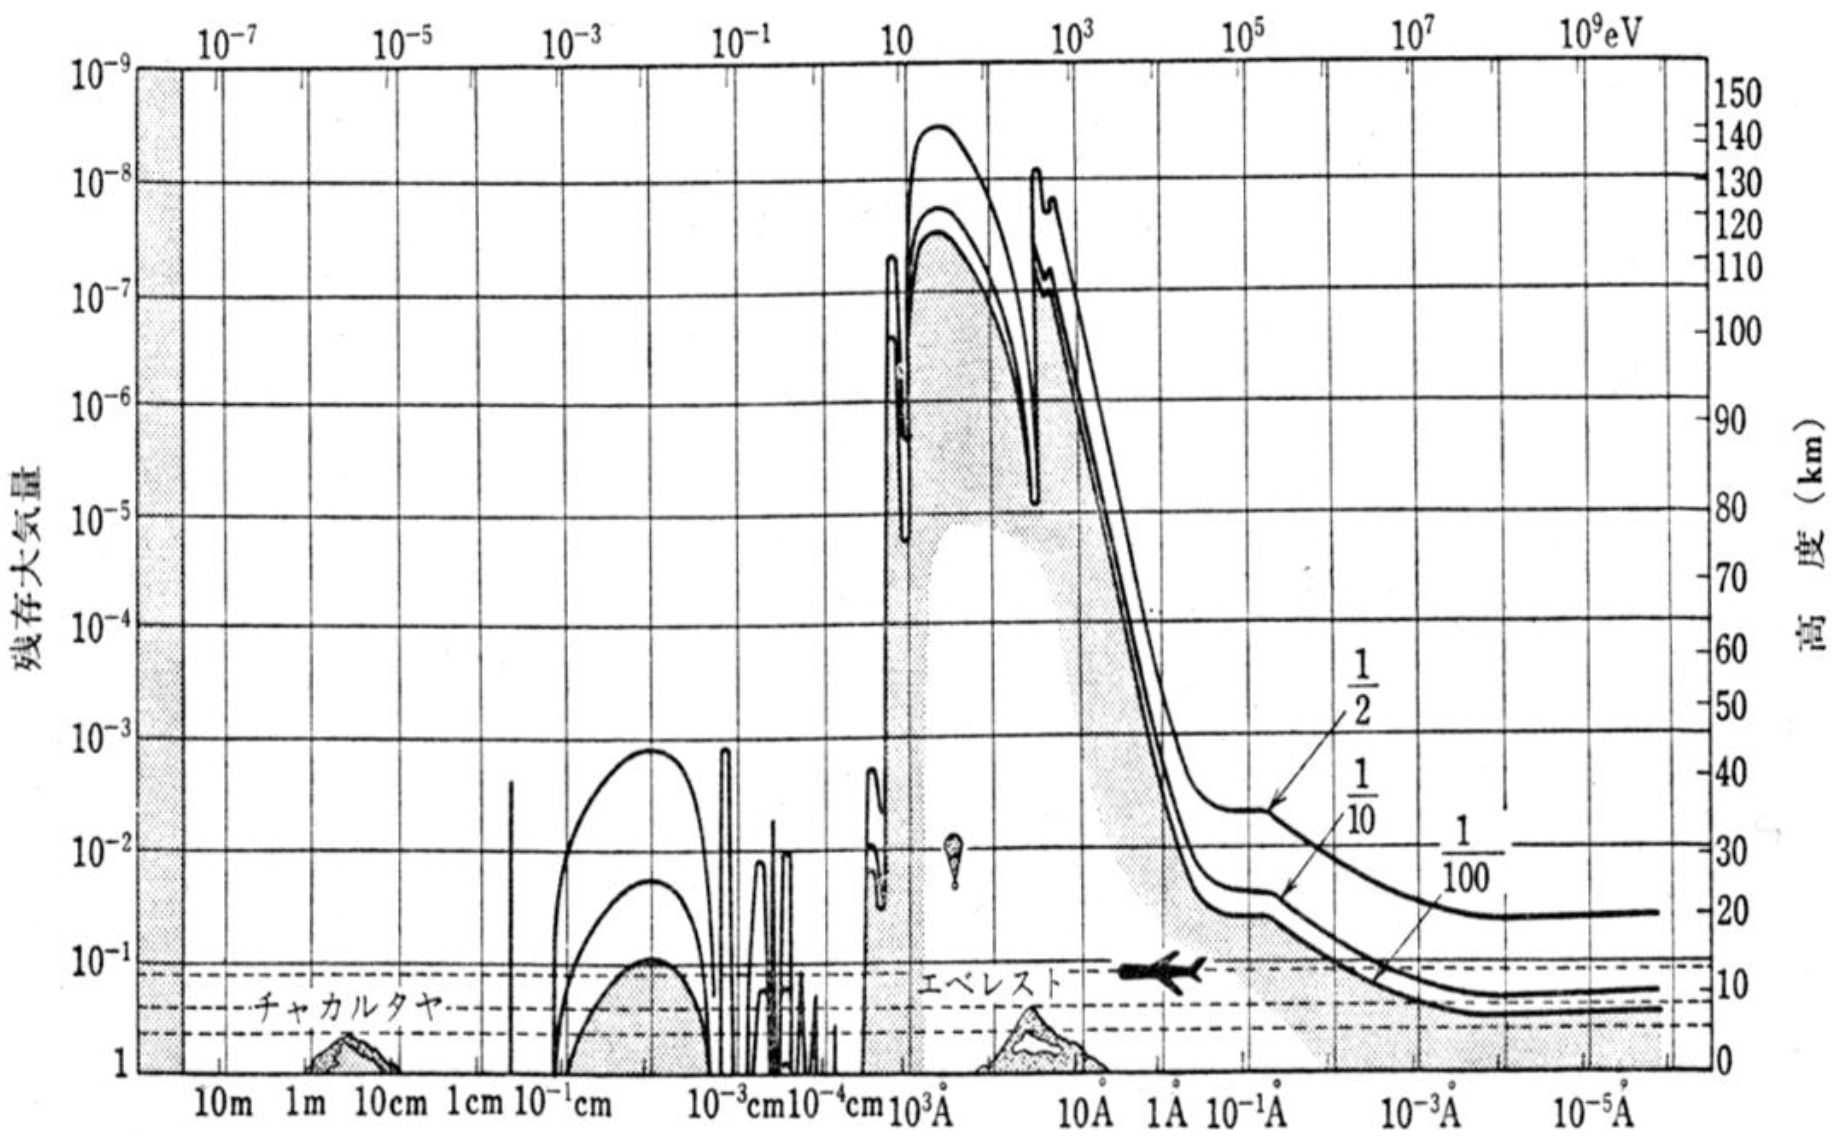
\includegraphics[width=15cm]{\PicPath/atmosphere_absorption.png}
\caption{大気による様々な波長の電磁波の吸収\cite{oda_and_matsuoka}}
\label{fig:atm_absp}
\end{figure}

%MeVガンマ線の観測には様々な困難を伴うため、あまり進んでいない
MeV領域は可視光やX線の領域に比べ、光子数が少なく透過力も高い上、物質との相互作用が主にコンプトン散乱によるので光子の完全な吸収は難しい。さらに銀河面全体に広がったガンマ線放射や、宇宙線と衛星本体との相互作用による大量のバックグラウンドが存在し、観測が非常に困難な領域である。以上の理由から、MeV領域の天文学は、他の波長域に比べ大きく遅れを取っているのが現状である。

この章ではMeVガンマ線領域について簡単に解説し、これまで行われてきたMeVガンマ線観測、そしてMeVガンマ線を観測することでどの様な物理現象の解明に繋がると期待されているかについて述べる。



%
天文学は色々なものを観測することで発展してきた
中でもMeVガンマ線というものは、観測することで〜〜といった物理現象の解明が期待されている
実際にMeVガンマ線を観測するためにCOMPTELだとかが上がったけどそんなに大きな成果は出していない(不十分)
この章では、MeVガンマ線観測によってどの様な物理事象の解明が期待されるかについて過去に行われてきた観測の結果を交えながら述べていく。


\section{これまでのMeVガンマ線天文学}
\subsection{MeVガンマ線領域}

画像だよ画像だよ画像だよ画像だよ画像だよ画像だよ画像だよ画像だよ画像だよ画像だよ画像だよ画像だよ画像だよ画像だよ画像だよ画像だよ画像だよ画像だよ画像だよ画像だよ画像だよ画像だよ画像だよ画像だよ画像だよ画像だよ画像だよ画像だよ画像だよ画像だよ画像だよ画像だよ画像だよ画像だよ画像だよ画像だよ画像だよ画像だよ画像だよ画像だよ画像だよ画像だよ画像だよ画像だよ画像だよ画像だよ画像だよ画像だよ画像だよ画像だよ画像だよ画像だよ画像だよ画像だよ画像だよ画像だよ画像だよ画像だよ画像だよ画像だよ画像だよ画像だよ画像だよ画像だよ画像だよ画像だよ画像だよ画像だよ画像だよ画像だよ画像だよ画像だよ画像だよ画像だよ画像だよ画像だよ画像だよ画像だよ画像だよ画像だよ画像だよ画像だよ画像だよ画像だよ画像だよ画像だよ画像だよ
\begin{figure}
\centering
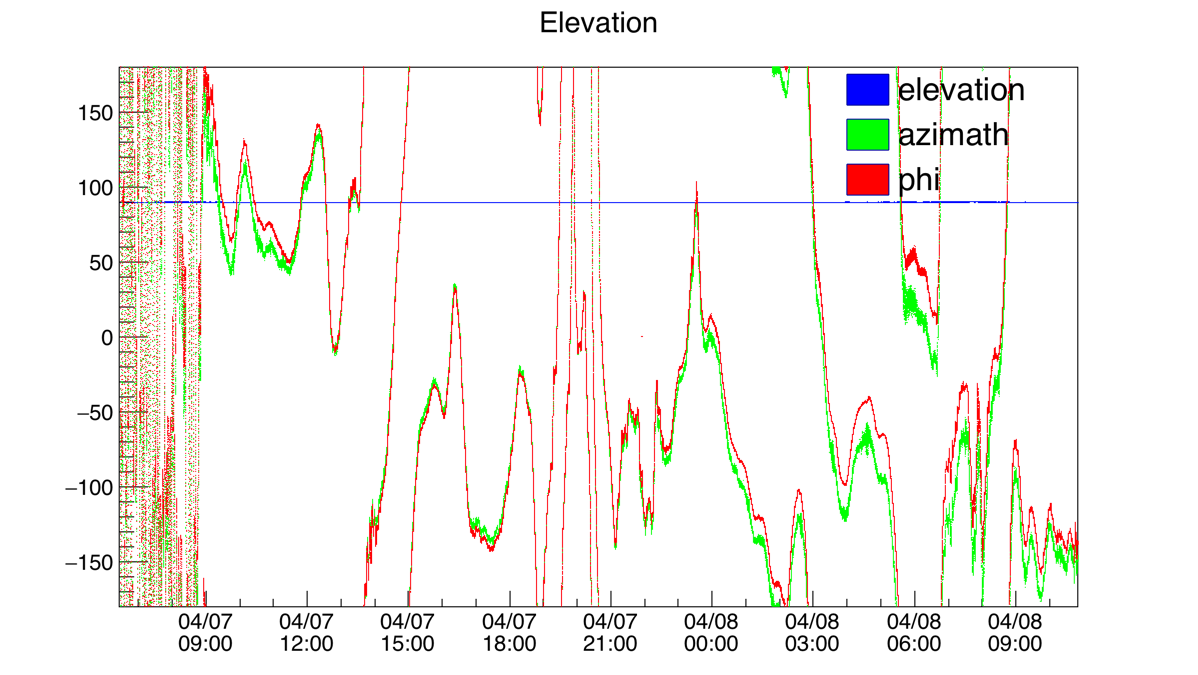
\includegraphics[width=15cm]{attitude_f.png}
\caption{test}
\end{figure}



%あとがき
 \backmatter
\chapter{あとがき}
ありがとうございました.

%参考文献(bibtex不使用で,手動で入力する場合.字下げの形式は『社会学評論スタイルガイド』にしたがっている)
\def\bibindent{1.85em}
\begin{thebibliography}{99\kern\bibindent}
\makeatletter
\def\@biblabel#1{}
\let\old@bibitem\bibitem
\def\bibitem#1{\old@bibitem{#1}\leavevmode\kern-\bibindent}
\makeatother
\small
\bibitem{}
Granovetter, Mark. 1973. ``The Strength of Weak Ties." \textit{American Journal of Sociology} 78(6): 1360--80.
\end{thebibliography}
\end{document}